%!TEX root = ../Pflichtenheft.tex

\chapter{Produktübersicht}
\label{chap:product_overview}
Um sich einen Überblick über die im Produkt enthaltenen Funktionen zu verschaffen, wird in diesem Kapitel eine Übersicht über die grundlegenden Funktionen in Form von Aktivitätsdiagrammen gegeben.
Zudem werden die Betriebsbedingungen beschrieben.
\section{Betriebsbedingungen}
\begin{itemize}
    \item Die Software soll in einem \gls{Docker}-\gls{Container} laufen.
    \item Die Software soll weitgehend ohne Unterbrechung laufen.
    \item Ständige Beobachtung ist nicht vorgesehen, die Software soll weitgehend autonom laufen.
    \item Übliche Administrationsaufgaben sollen über die Administrationsoberfläche und ohne Neustart der Software möglich sein.
    \item Die \gls{RAM}-Nutzung soll möglichst gering sein (Ideal: unter 1GB)
\end{itemize}

\newpage
\section{Aktivitätsdiagramm-Diagramme}

\subsection{Admin Funktionalität}
In Abbildung \ref{fig:activity_diagram_admin} ist das Aktivitätsdiagramm für die Admin-Funktionalität dargestellt.
\begin{figure}[ht]
    \centering
    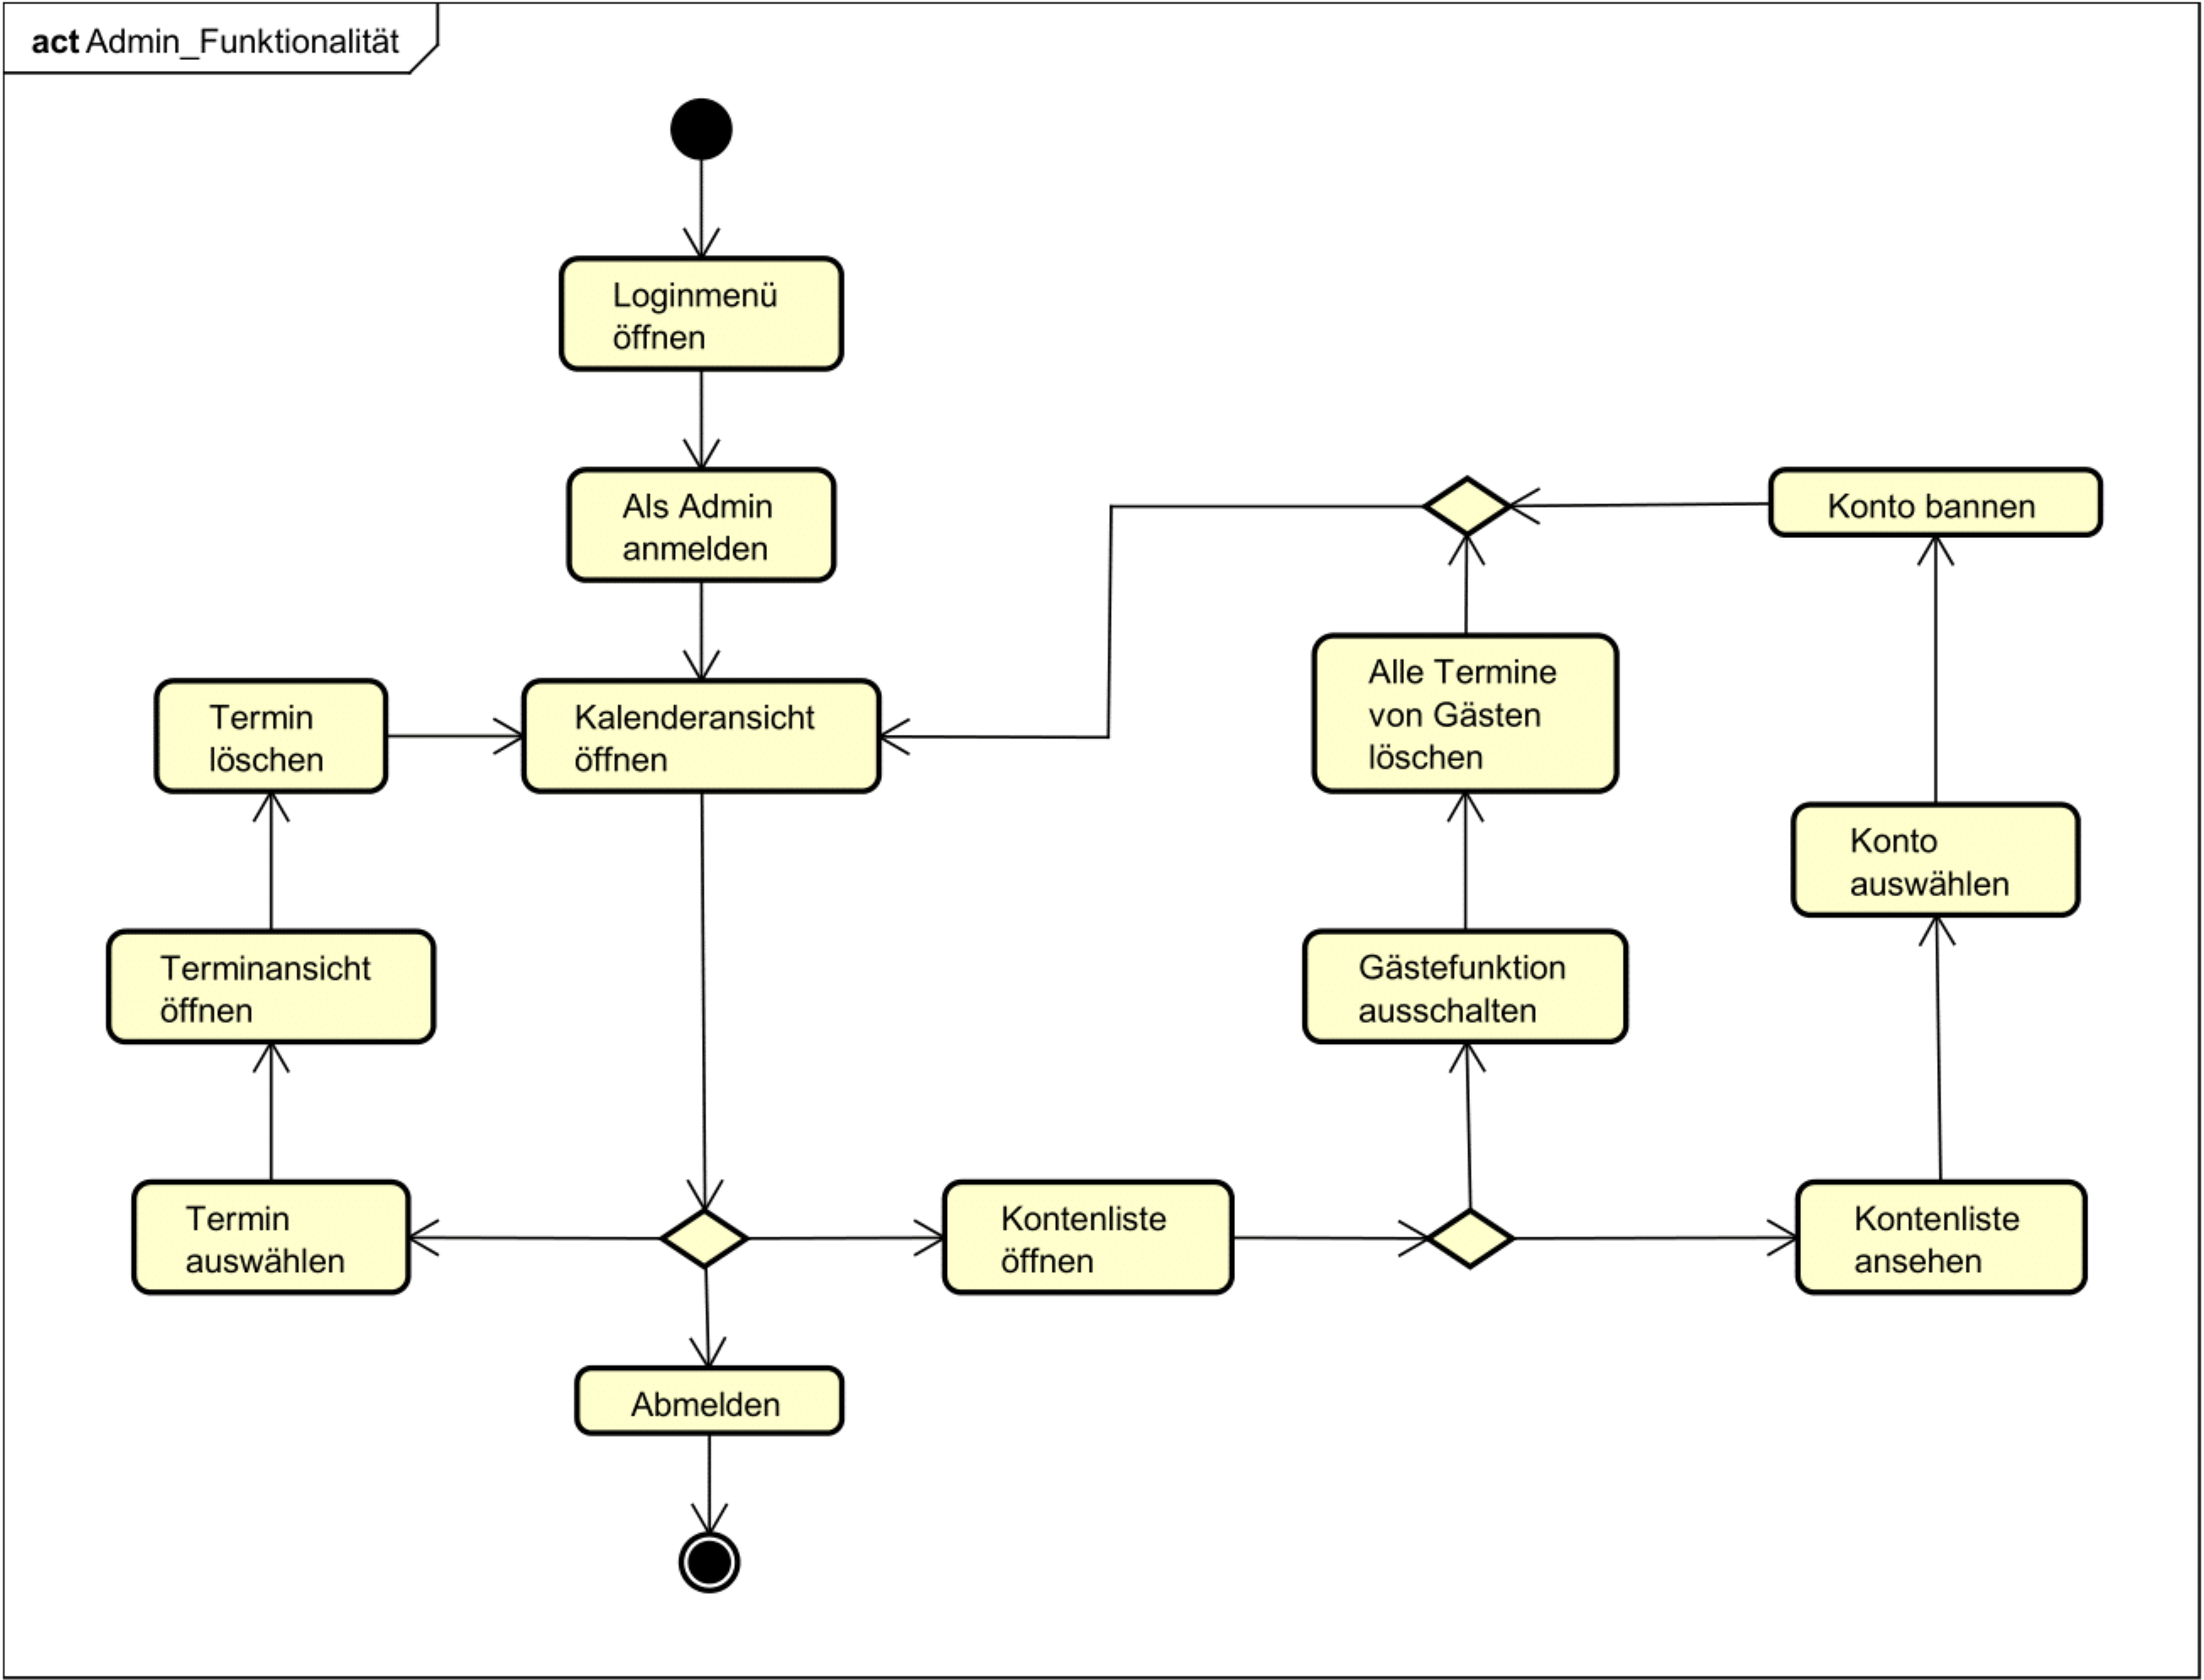
\includegraphics[width=\textwidth]{figures/activitydiagrams/adminfunk}
    \caption{Aktivitätsdiagramm für die Admin-Funktionalität}
    \label{fig:activity_diagram_admin}
\end{figure}
\clearpage
\subsection{Anmeldeprozess}

In Abbildung \ref{fig:activity_diagram_login} ist das Aktivitätsdiagramm für den Anmeldeprozess dargestellt.
\begin{figure}[ht]
    \centering
    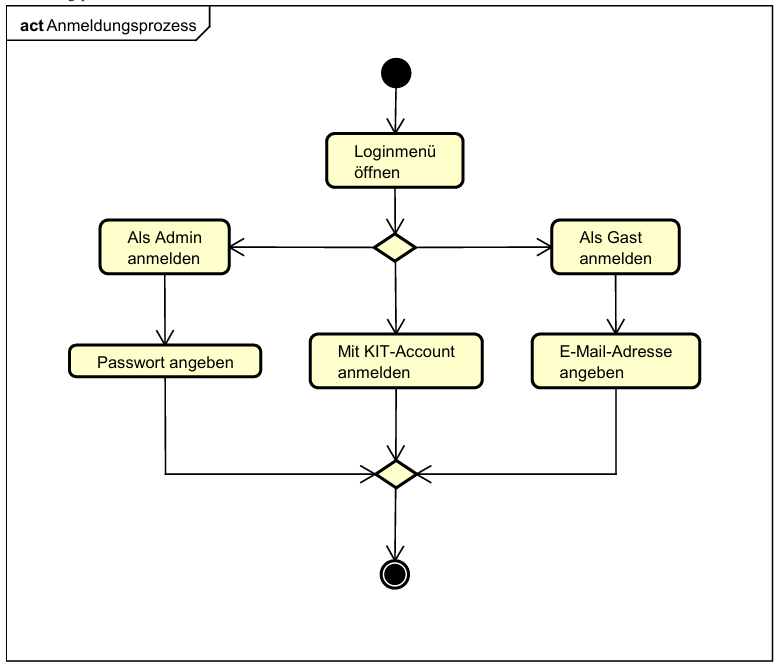
\includegraphics[width=\textwidth]{figures/activitydiagrams/anmeldeprozess}
    \caption{Aktivitätsdiagramm für den Anmeldeprozess}
    \label{fig:activity_diagram_login}
\end{figure}
\clearpage
\subsection{Termin erstellen}

In Abbildung \ref{fig:activity_diagram_booking} ist das Aktivitätsdiagramm für das Erstellen eines Termins dargestellt.
\begin{figure}[ht]
    \centering
    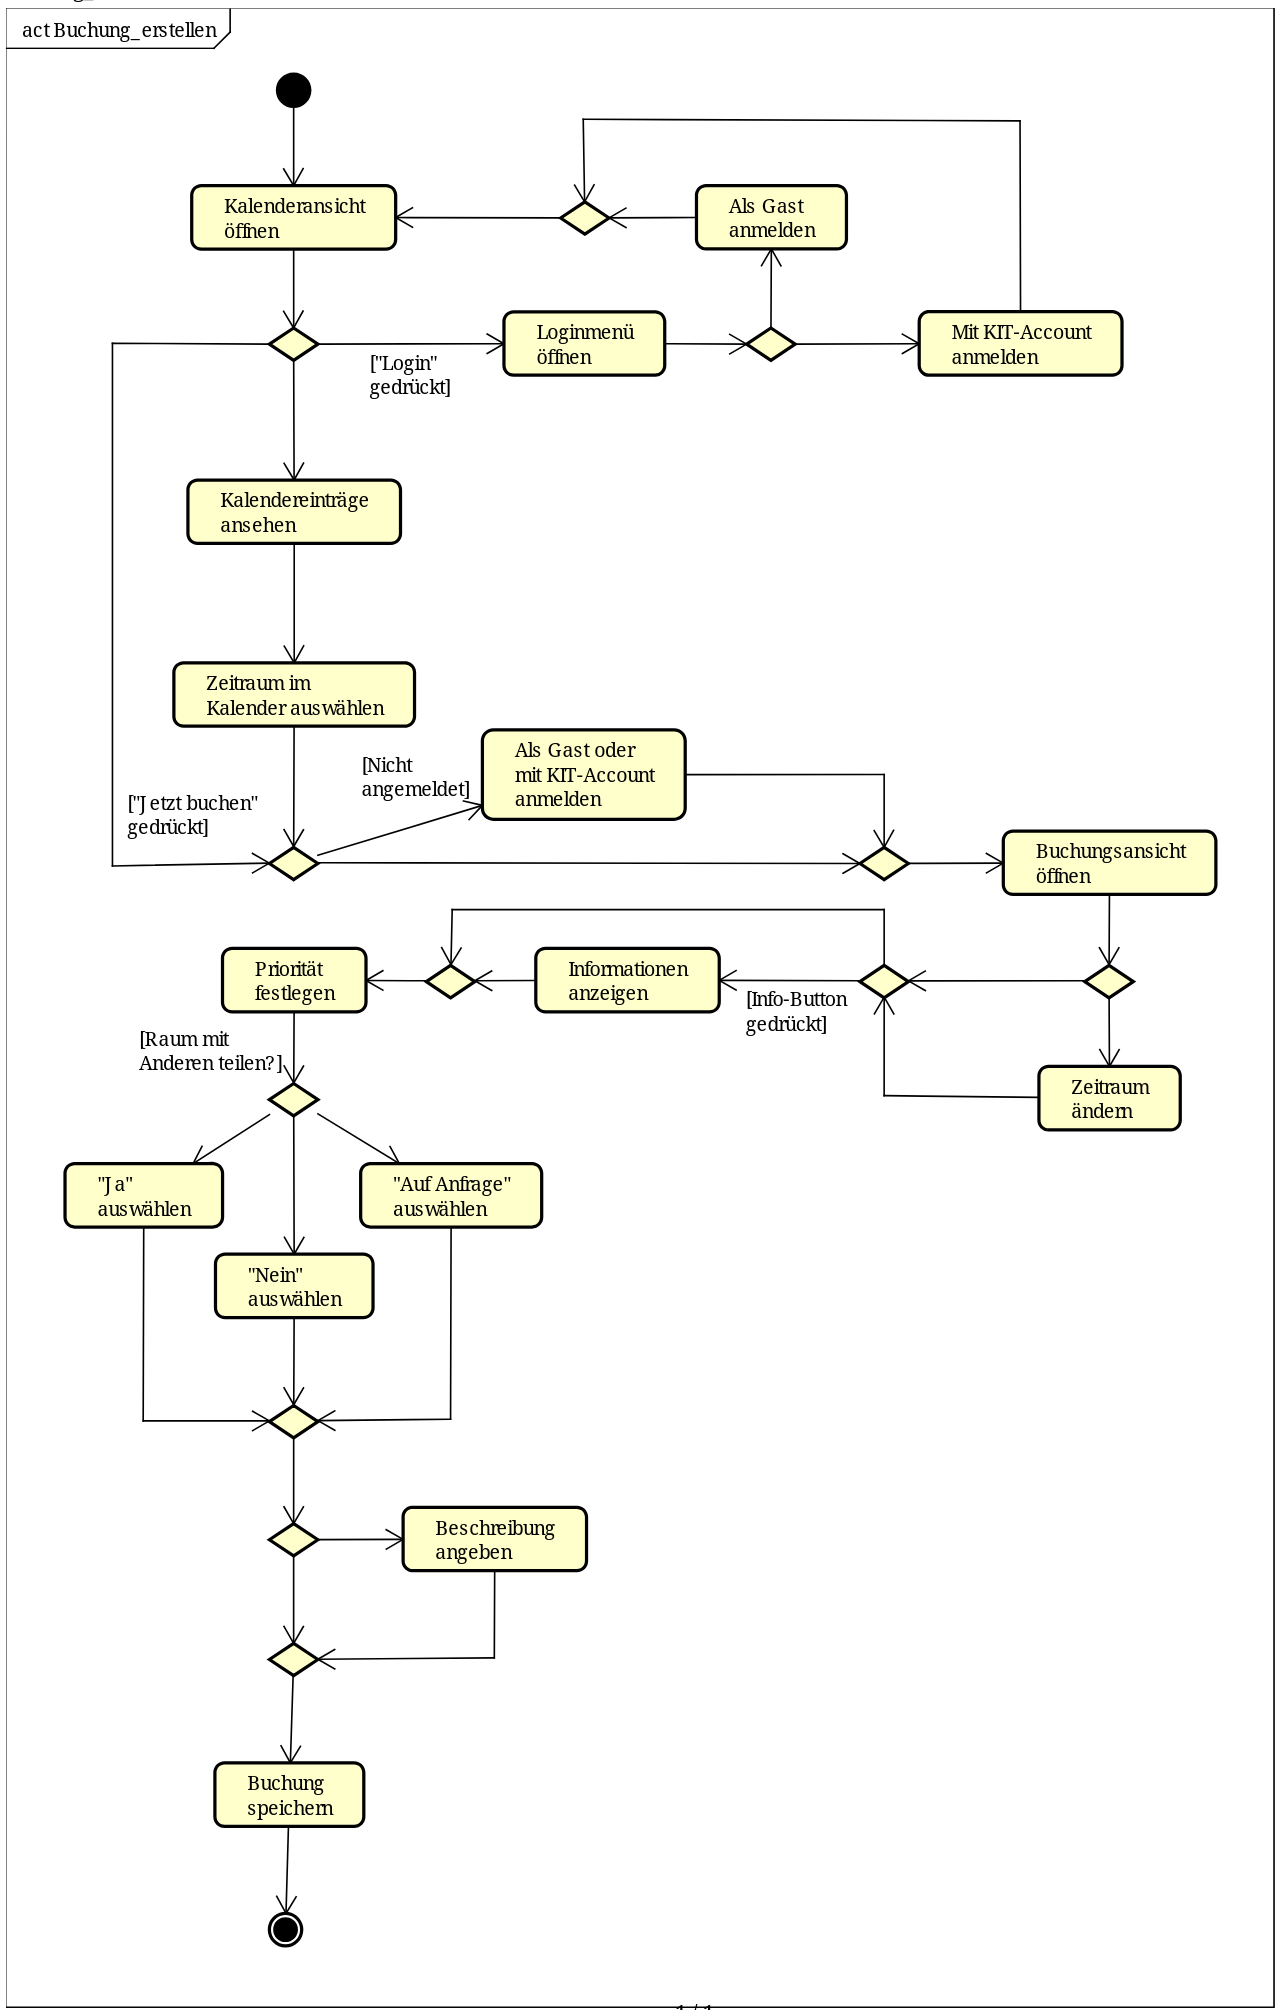
\includegraphics[width=0.6\textwidth]{figures/activitydiagrams/buchungerstellen}
    \caption{Aktivitätsdiagramm für das Erstellen eines Termins}
    \label{fig:activity_diagram_booking}
\end{figure}


\clearpage
\subsection{Termine verwalten}
In Abbildung \ref{fig:activity_diagram_booking_manage} ist das Aktivitätsdiagramm für das Verwalten von Terminen dargestellt.
\begin{figure}[ht]
    \centering
    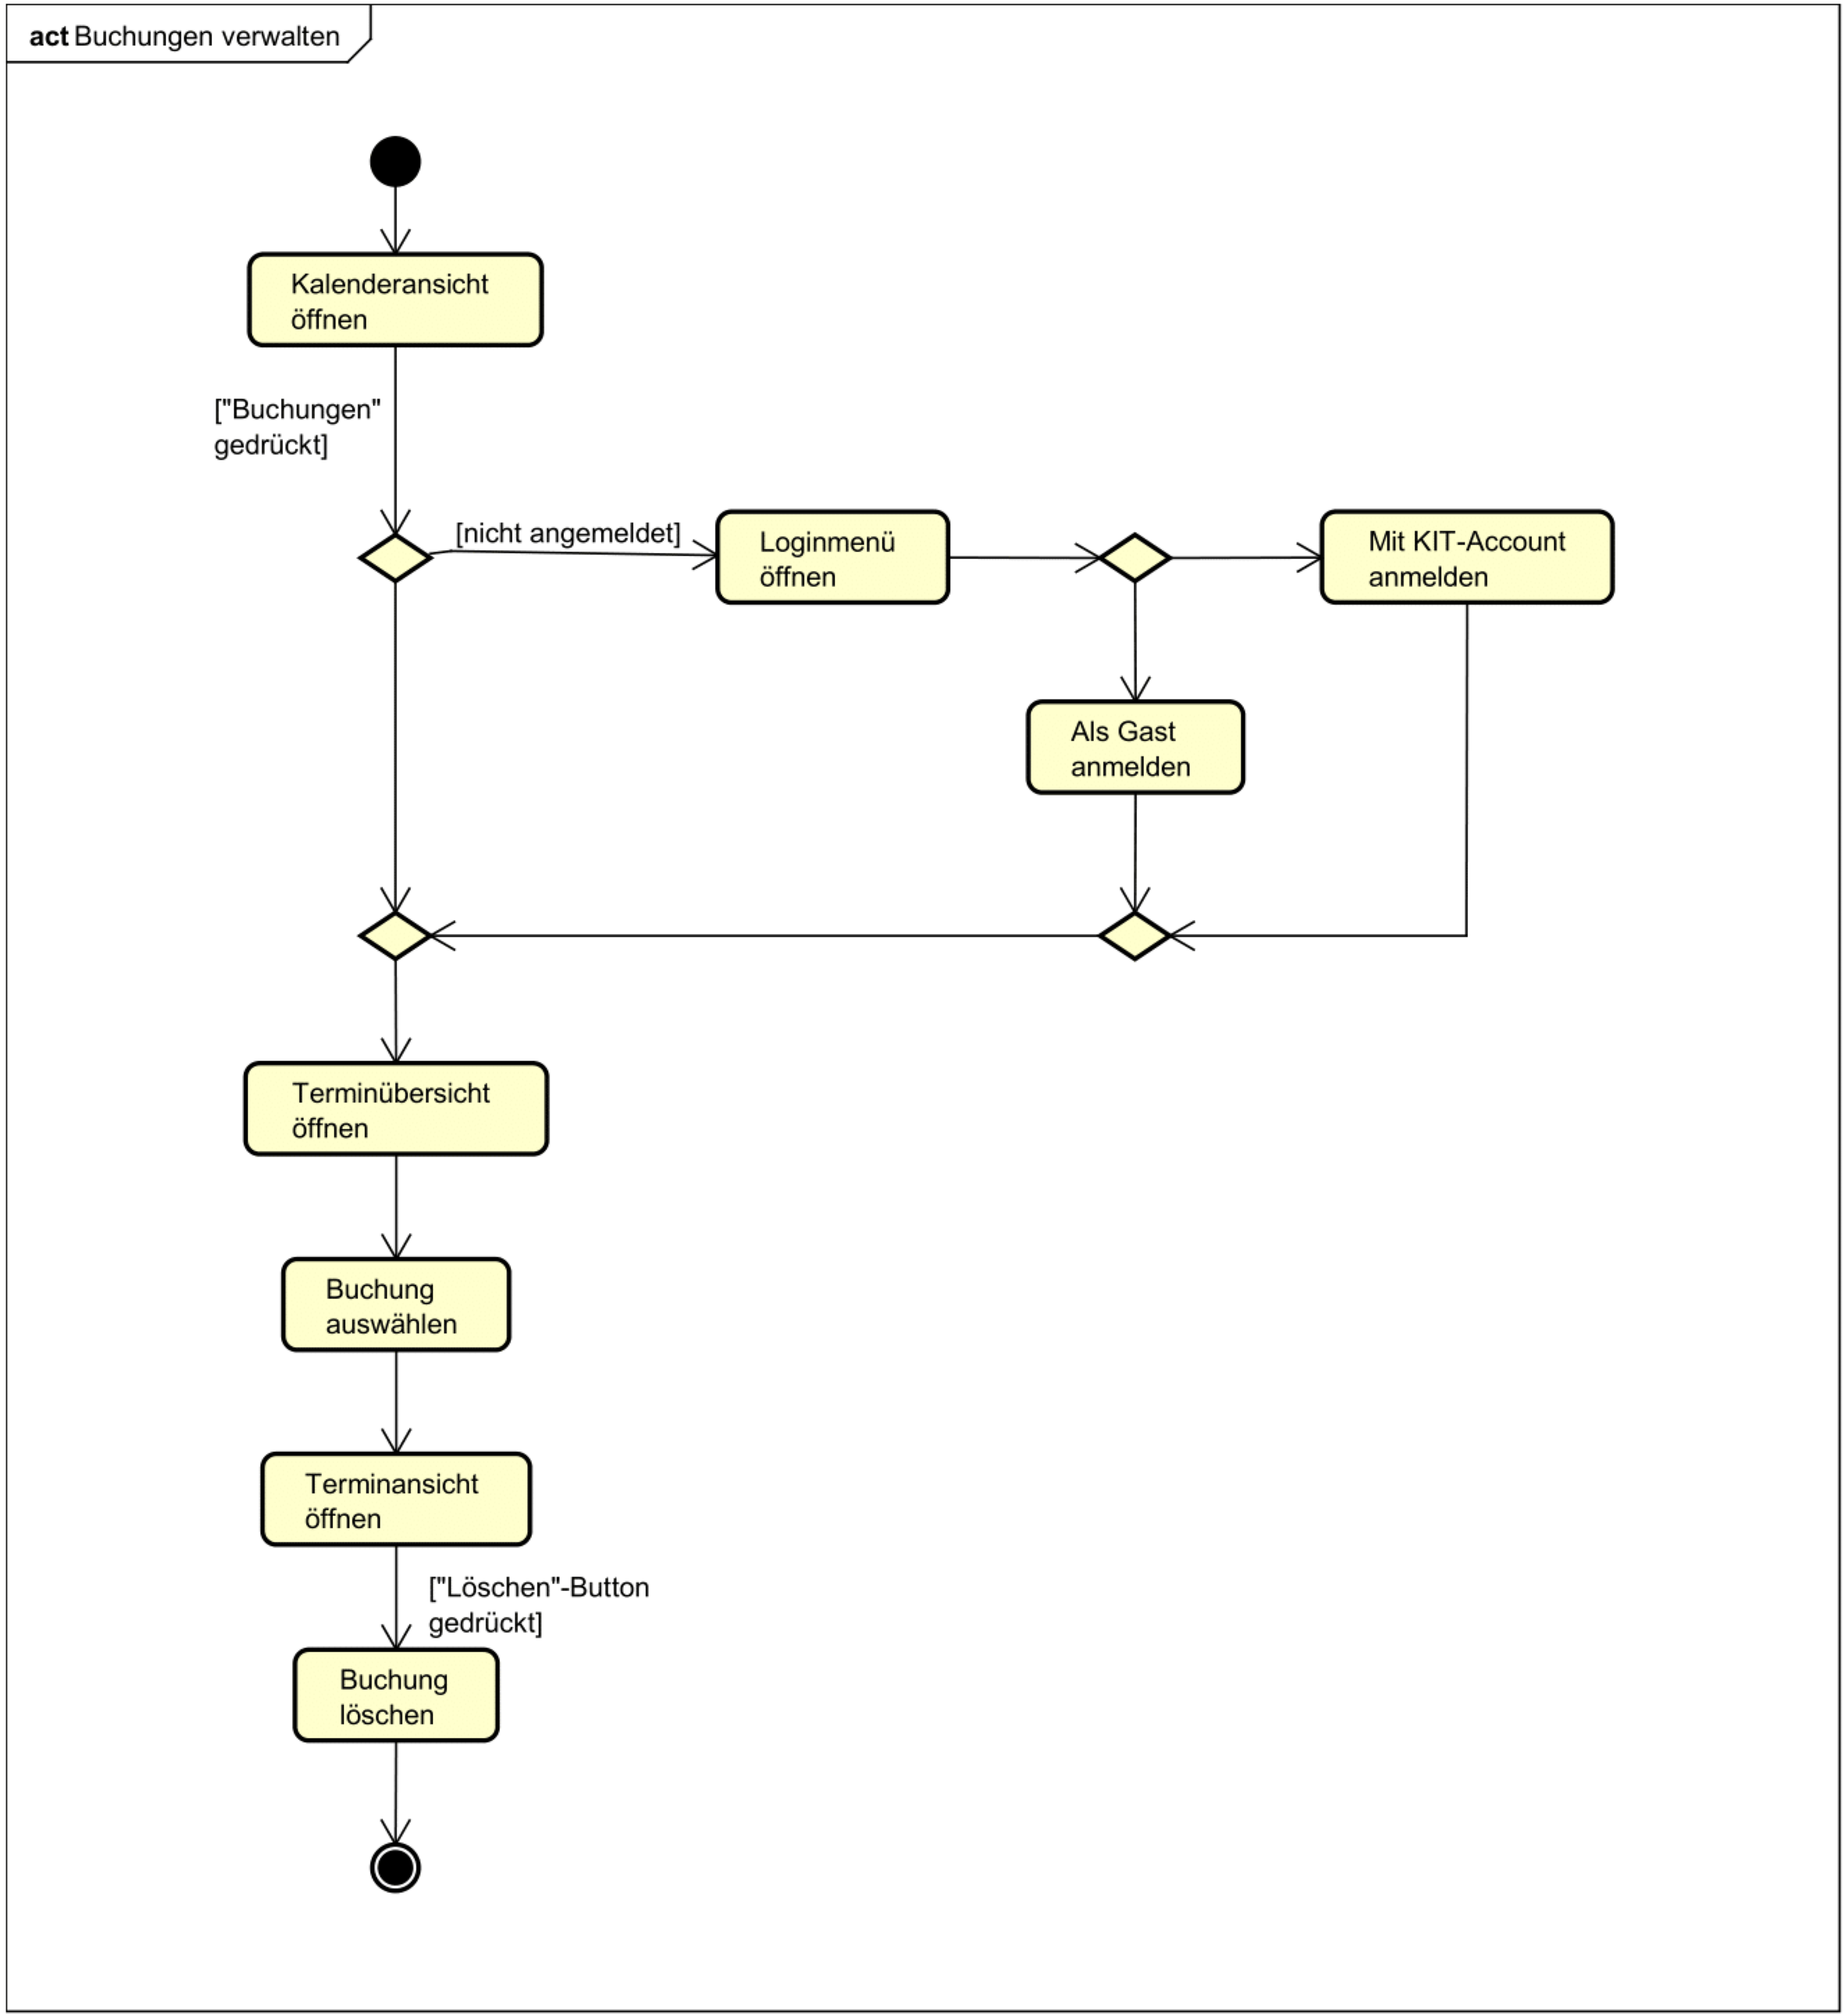
\includegraphics[width=0.8\textwidth]{figures/activitydiagrams/buchungverwalten}
    \caption{Aktivitätsdiagramm für das Verwalten von Terminen}
    \label{fig:activity_diagram_booking_manage}
\end{figure}

\clearpage
\subsection{Termin Ansicht}
In Abbildung \ref{fig:activity_diagram_calendar} ist das Aktivitätsdiagramm für die Ansicht <Termin> dargestellt.
\begin{figure}[ht]
    \centering
    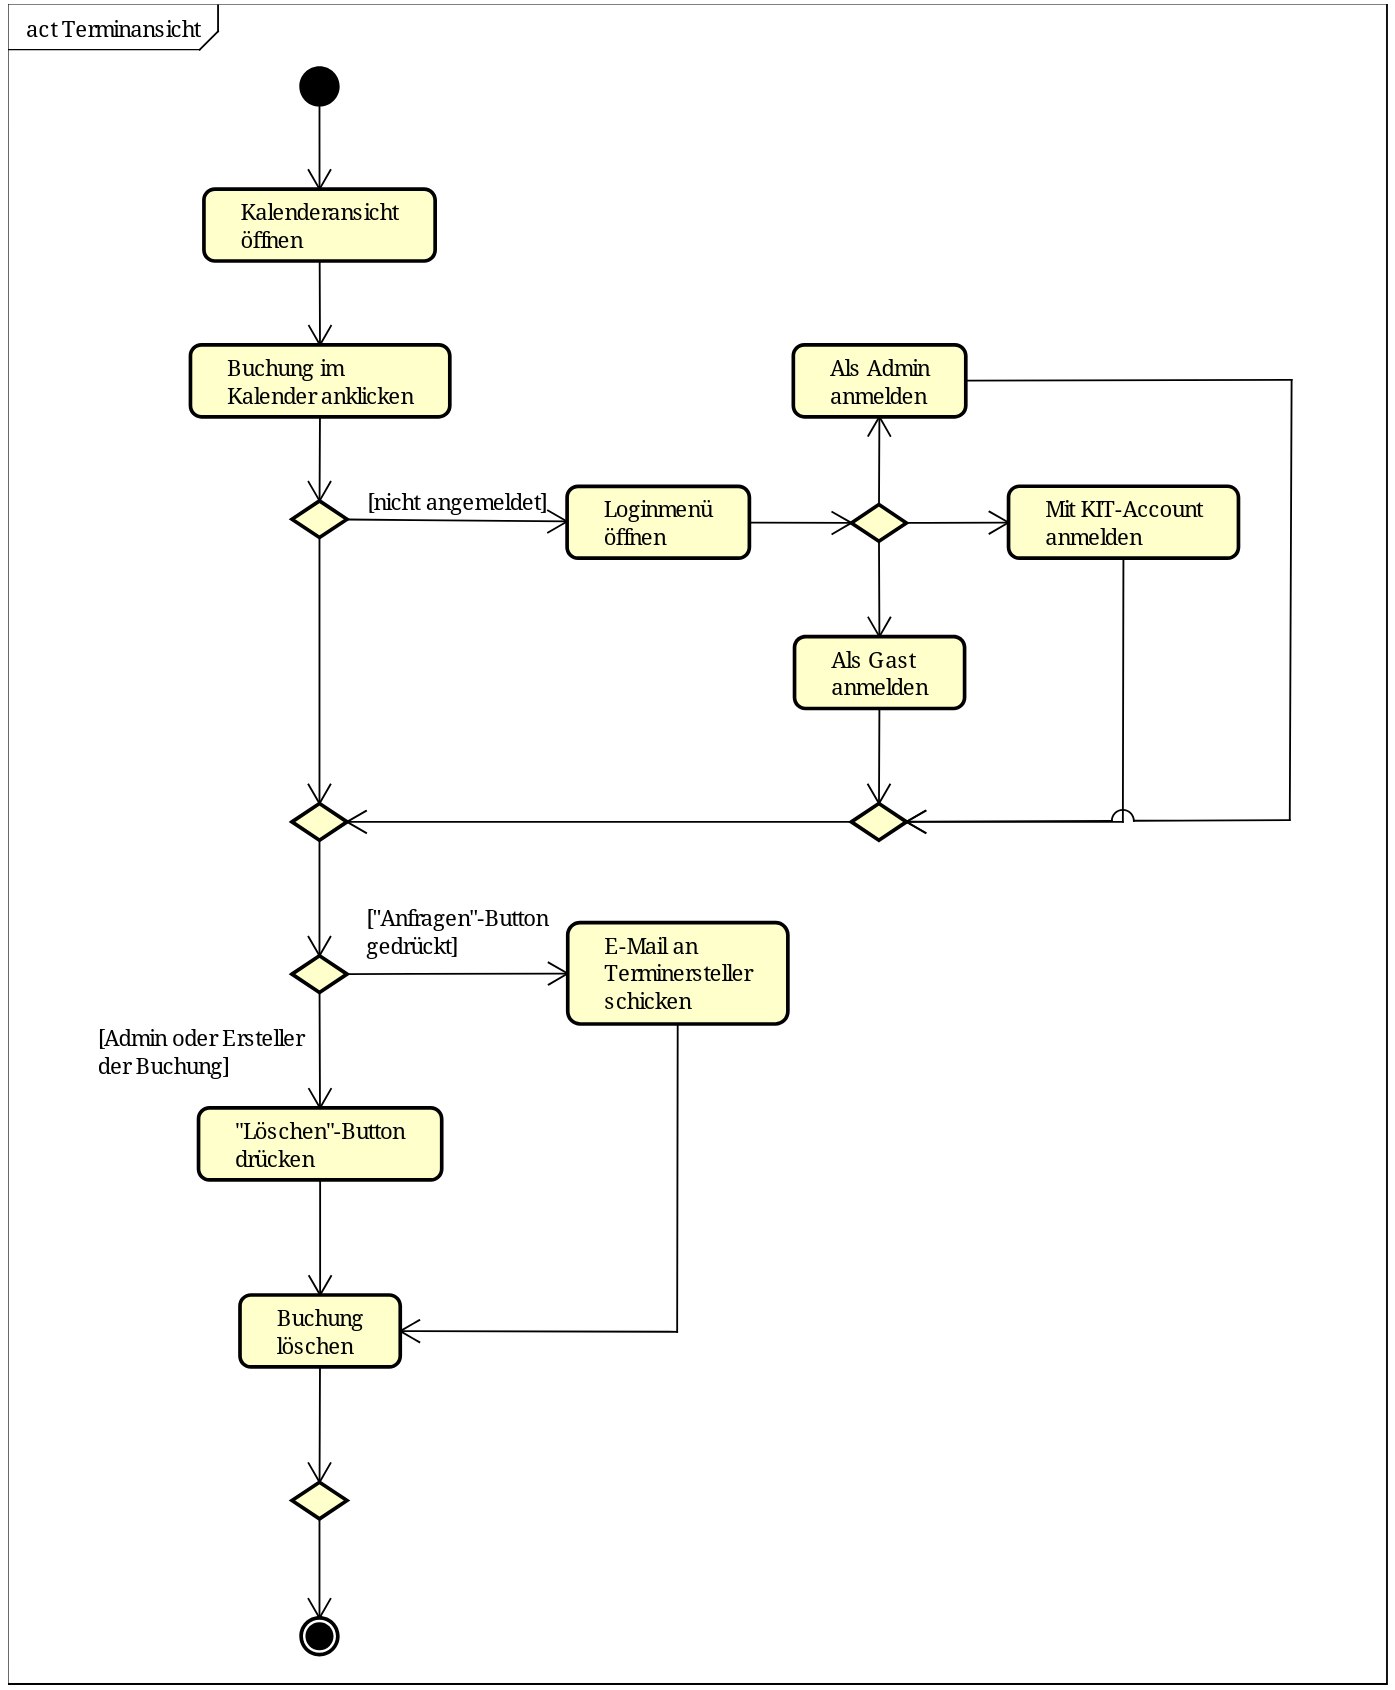
\includegraphics[width=0.8\textwidth]{figures/activitydiagrams/terminansicht}
    \caption{Aktivitätsdiagramm für die Ansicht <Termin>}
    \label{fig:activity_diagram_calendar}
\end{figure}